\documentclass{article}
\usepackage[utf8]{inputenc}
\usepackage{fancyvrb}
\usepackage{graphicx}
\usepackage{float}
\usepackage[portuges]{babel}
\usepackage[colorlinks]{hyperref}

\begin{document}
\title{\textbf{Reverse Proxy}}
\author{João Pedro Ferreira Vieira\\
		A78468@alunos.uminho.pt \and
		José Carlos Lima Martins\\
        A78821@alunos.uminho.pt \and
        Miguel Miranda Quaresma\\
        A77049@alunos.uminho.pt}
\date{Universidade do Minho\\
	  Comunicação por Computadores\\[2ex]%
      \today}
\maketitle

\begin{abstract}
Após a implementação de um serviço de distribuição de carga com servidor proxy, procedemos à documentação do mesmo, de modo a ser perceptível o que foi desenvolvido. Inicialmente é apresentada a arquitetura da solução proposta bem como os formatos dos pacotes sendo, de seguida, explicada a implementação e apresentados os testes e os resultados obtidos.
\end{abstract}

\section{Introdução}
O trabalho desenvolvido tem como objetivo a implementação de um serviço de distribuição de carga com servidor proxy invertido usado quando há a necessidade de mais do que um servidor a atender vários clientes devido ao grande volume dos mesmos e pretende-se manter um único endereço IP público.

\section{Arquitetura da solução}
Pretende-se implementar um serviço de distribuição de carga com servidor proxy invertido, no qual existe um servidor com um endereço IP público(o reverse proxy) que atende todos os clientes, direccionando-os para um dos servidores HTTP de back-end disponíveis. 
É importante referir é que no nosso trabalho as conexões dos clientes não são desviadas sendo criado um ``túnel'' no Reverse Proxy entre o servidor HTTP de back-end escolhido e o cliente. Esta decisão foi tomada devido à menor complexidade envolvida na sua implementação representando, no entanto, um ponto de falha grave no Reverse Proxy.
O sistema desenvolvido pode ser dividido em 3 componentes princpais: MonitorUDP, tabela de estado e o ``Reverse Proxy''. 

O MonitorUDP envia, em Multicast, um datagrama UDP de 3 em 3 segundos para todos os agenteUDP's (um por cada servidor HTTP back-end) estes respondem depois, em Unicast, com informação relativa ao estado do servidor a que se encontram assocaidos. O MonitorUDP, ao receber um datagrama UDP de um dos agenteUDP's, calcula o RTT(Round Trip Time), obtém o IP e porta de origem do datagrama e atualiza a tabela de estado referente ao servidor HTTP back-end do qual foi recebido o datagrama.

A tabela de estado possui, em cada linha, informação referente a um único servidor HTTP back-end, sendo que esta informação é organizada da seguinte maneira:

\begin{verbatim}
IP;;Porta;;CPU_usado;;RAM_livre;;RTT;;BW(bandwidth)
\end{verbatim}
em que o 3º parâmetro (CPU\_usado) é uma percentagem, a RAM\_livre corresponde a quantidade de memória em bytes, o RTT representa um intervalo de tempo em milisegundos, e a BW (bandwidth) é um tamanho em Kbytes por segundo (Kbps).

Quanto ao ``Reverse Proxy'' quando este recebe um pedido de conexão de um cliente, tem que escolher, com recurso a um algoritmo pré-estabelecido,  um servidor HTTP (da tabela de estado anteriormente referida), criar uma ligação TCP entre o mesmo(servidor HTTP) e o cliente e atualizar, periodicamente, o valor da bandwidth para esse servidor.

A arquitetura descrita encontra-se ilustrada na seguinte figura:
\begin{figure}[H]
	\centering
	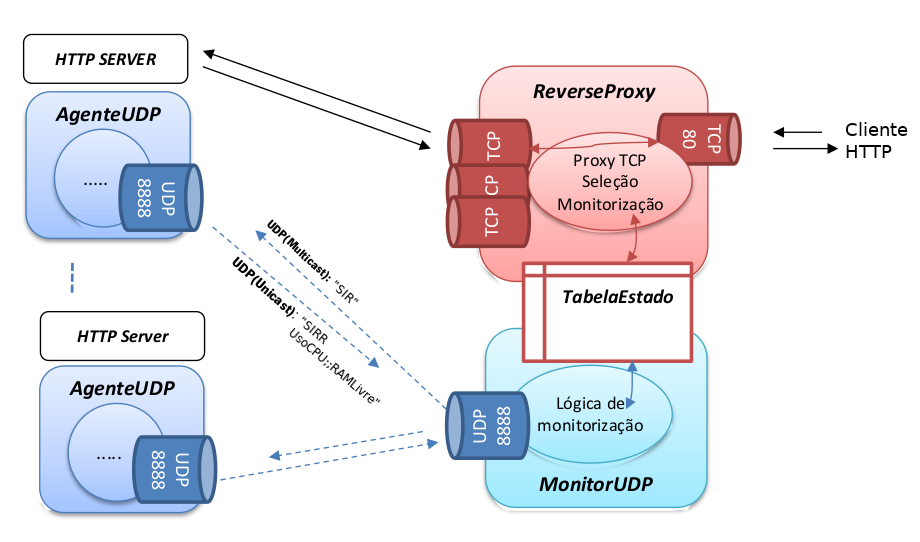
\includegraphics[height=6cm]{arquitetura.png}
\end{figure}

\section{Especificação do protocolo UDP}

\subsection{Formato das mensagens protocolares (PDU)}
As mensagens trocadas entre os UDPAgent's e o UDPMonitor são de dois tipos: 
\begin{itemize}
    \item mensagens enviadas pelo UDPMonitor, em Multicast, para todos os UDPAgent's
    \item mensagens de cada UDPAgent, quando recebe a mensagem do UDPMonitor, para o mesmo em Unicast
\end{itemize}

A mensagem enviada do UDPMonitor para todos os membros do grupo Multicast tem o intuito de pedir informação referente ao estados dos servidores HTTP e, como tal, possui um formato simples sendo o seu conteúdo a seguinte \texttt{String}: ``SIR''.
Já a mensagem unicast, de cada UDPAgent para o UDPMonitor em resposta à mensagem anteriormente descrita contém toda informação referente ao estado de um dado serivdor HTTP e, como tal, apresenta o seguinte formato:
\begin{verbatim}
SIRR
percentagem_de_uso_do_CPU;;memoria_RAM_livre
\end{verbatim}
De notar que a \texttt{String} ``;;'' é usada como separador dos diferentes campos que constituem a mensagem. 

\subsection{Interações}
Como é possível observar são estabelecidas várias interações entre os intervenientes do sistema desenvolvido, nomeadamente entre:
\begin{description}
    \item [UDPAgent e UDPMonitor] O UDPMonitor envia, em \textit{multicast}, para todos os UDPAgent's no grupo a mensagem "SIR", estes respondem à mesma em \textit{unicast} com os valores do servidor em que estão a correr, de forma a poder ser atualizada a sua informação na Tabela de Estados do programa. É importante referir que a autenticidade e integridade das mensagens trocadas entre estes dois intervenientes é garantida.
    \item [UDPMonitor e StateTable] Sempre que o UDPMonitor recebe informações dos servidores através dos UDPAgent's cabe-lhe a função de atualizar os valores destes servidores na Tabela de Estados caso estes já sejam pertencentes ou grupo, ou simplesmente adicionar um novo servidor com a sua respetiva informação 
à tabela em causa.
    \item [Cliente e ReverseProxy] Quando um cliente requisita uma consulta ao ReverseProxy este escolhe o melhor servidor no devido momento tendo em conta os valores dos mesmos na Tabela de Estados (cálculo através do algoritmo) e cria um "túnel" entre esse mesmo servidor e o cliente de forma a estabelecer a conexão necessária.
    \item [ReverseProxy e StateTable] Cabe ao ReverseProxy calcular a \textit{bandwidth} sempre que um cliente faça um \textit{download} através de um dos servidores disponíveis. Com isto, cabe ao ReverseProxy atualizar o valor da \textit{bandwidth} desse mesmo servidor na Tabela de Estados tendo em conta o valor calculado.
\end{description}


\section{Implementação}
O trabalho foi desenvolvido utilizando a linguangem de programação Java e, como tal, decidimos dividir o código pelas seguintes classes:
\begin{description}
    \item [StateTable] Representa a tabela de estados
    \item [UDPMonitor] Envia datagramas UDP de 3 em 3 segundos para o canal multicast 
    \item [UDPAgent] Responde em unicast ao MonitorUDP com o estado do servidor HTTP a que está associado
    \item [ListenUDPAgents (Thread do UDPMonitor)] Recolhe os datagramas enviados pelos UDPAgent's e atualiza com estes diagramas a tabela de estados (StateTable)
    \item [Timer] Usado pelo UDPMonitor e pelo ListenUDPAgents de modo a calcular o RTT das ligações com os servidores
    \item [ReverseProxy] O Reverse Proxy funciona como um servidor TCP recebendo pedidos na porta 80 dos clientes
    \item [Connection (Thread do ReverseProxy)] criada para tratar de cada cliente, ou seja cada cliente possui uma Thread Connection no ReverseProxy sendo que esta Thread trata de escolher o servidor HTTP da tabela de estados, inicia a Thread ListenFromClient e fica à escuta do servidor HTTP e envia os dados para o cliente
    \item [ListenFromClient (Thread da Connection)] Envia os dados que recebe do cliente para o servidor HTTP
\end{description}

Tanto a classe Timer bem como a StateTable foram implementadas tendo em mente o controlo de acesso concorrentes nomeandamente com recurso a lock's de modo a impedir que Threads/Processos diferentes tenham acesso simultaneo aos dados, evitando assim race conditions como dead lock's inconsistências nos dados.

A biblioteca Sigar, da Hyperic, permite-nos obter dados como a percentagem de uso de CPU e de memória livre do sistema(com UDPAgent e servidor HTTP) e não apenas o que a máquina virtual do Java(JVM) disponibilizou para a execução do UDPAgent. De realçar que esta biblioteca é cross-platform \textbf{i.e.} funciona em vários sistemas operativos. Contudo é importante salientar que, dado os testes efetuados serem realizados na máquina, os dados obtidos pelos vários UDPAgent's é o mesmo. Desta biblioteca foram usado as seguintes funcionalidades:
\begin{itemize}
	\item org.hyperic.sigar.Sigar: necessário de modo a poder usar as funcionalidades seguintes
	\item org.hyperic.sigar.Mem: permite a obtenção de dados referentes à memória RAM
	\item org.hyperic.sigar.Cpu: permite a obtenção de dados referentes ao CPU
\end{itemize}
Já em relação às bibliotecas predefinidas do Java destacam-se as que permitem a conexão entre os diferentes componentes, tanto por TCP como por UDP, e as que nos permite garantir a integridade bem como autenticação dos pacote:
\begin{itemize}
	\item java.net.DatagramPacket: permite a criação de datagramas UDP
  	\item java.net.DatagramSocket: permite a criação de sockets UDP
    \item javax.crypto.Mac: permite o uso do algoritmo \textbf{HMAC} modo a garantir integridade e autenticação dos pacotes transferidos entre UDPAgent's e UDPMonitor
    \item java.net.InetAddress: representa um endereço IP
    \item javax.crypto.spec.SecretKeySpec: permite a criação de uma chave a partir de um conjunto de bytes (que podem ser obtidos convertendo uma String para um array de bytes)
    \item java.net.ServerSocket: permite a criação de um servidor TCP que pode aceitar conexões de clientes numa determinada porta
	\item java.net.Socket: permite a criação de sockets TCP
    \item java.net.MulticastSocket: permite a criação de um grupo Multicast
\end{itemize}

O algoritmo usado na escolha do servidor HTTP (para um dado cliente) por parte do Reverse Proxy tem em conta os valores armazenados na StateTable nomeadamente: percentagem de memória livre, percentagem de CPU usado, RTT e bandwidth(banda larga). O peso associado a cada um dos parâmetros é de 25\%(1/4=0.25). Por forma a que todos os parametros tenham efetivamente o mesmo peso no algoritmo de escolha é necesário garantir que todos sejam valores percentuais. Para tal o RTT é dividido por 3000 ms (3s, o tempo entre datagramas enviados pelo UDPMonitor), a memória livre e a bandwidth são divididas pelo valor máximo já encontrado para cada um dos campos garantindo que os valores se encontrão sempre entre 0 e 1. A seguinte fórmula é aplicada a cada linha da tabela:
\begin{verbatim}
res = 0.25 * percentagem_de_uso_do_CPU - 0.25 * memoria_RAM_livre / maxRAM 
	+ 0.25 * RTT / 3000 + 0.25 * BW / maxBW;
\end{verbatim}
e foi pensada de forma a que o servidor ótimo seja o que apresente o menor valor de todos os presentes na tabela.

Para garantir a autenticidade e a integridade das mensagens trocadas entre o UDPMonitor e o UDPAgent é usada uma chave conhecida tanto pelo Monitor como pelos Agent's, esta chave é uma \texttt{String} arbitrária e com o valor de "\textbf{abcdfasdgasefdgsdp}". A partir daqui, e supondo que \texttt{msg} é o conteúdo que é necessário ser enviado do UDPAgent para o UDPMonitor, acrescentamos no início desta mesma mensagem a \texttt{hash} associada à mensagem e à chave acima indicada, esta \texttt{hash} é obtida com recurso ao algoritmo SHA256 que gera uma \texttt{hash} de 256bits ou 32 bytes. Desta forma, o pacote enviado pelo UDPAgent ao UDPMonitor é "\texttt{hash} (32 bytes) + \texttt{msg}". Quando este mesmo pacote é recebido pelo UDPMonitor, este extrái o mesmo para um conjunto de bytes, e separa a \texttt{hash} da \texttt{msg}. Após, isto, calcula uma nova \texttt{hash} da \texttt{msg} tendo em conta a chave que partilhada entre o mesmo e o UPDAgent e compara o mesmo com o valor de \texttt{hash} extraído anteriomente, caso o valor seja o mesmo garante-se tanto a autenticidade como a integridade da mensagem recebida.

O cálculo da bandwidth ofereceu alguns obstáculos na obtenção de um valor representativo sendo que uma das decisões tomadas nestes sentido foi a adição da bandwidth (BW) da ligação (tanto entre cliente-ReverseProxy como entre servidor HTTP-ReverseProxy) num dado instanto ao valor presente na tabela de estados. Porém esta abordagem apresentava um problema, visto que, a bandwidth iria aumentar indefinidamente, algo que não acontece na realidade. Este problema é resolvido guardando valor da bandwidth anterior (prevBW) e, na altura da adição, em vez de se adicionar BW adiciona-se (BW-prevBW). Para além disso, de modo a que, quando uma determinada ligação caia esta não mantenha o valor da bandwidth na tabela (visto a mesma já não ter influência no mesmo), subtrai-se BW ao valor existente na tabela de estados. Apesar de tudo a abordagem descrita apresentava ainda um problema, visto que a maior parte das vezes a bandwidth era igual a 0 algo justificado pelo pequeno intervalo de tempo e pequeno número de bytes usado para calcular a bandwidth. Sendo assim, em vez de este ser calculado a cada 1024 bytes passa a ser calculado de 20 em 20 ciclos de 1024 bytes. A fórmula usada para calcular a bandwidth é a seguinte:
\begin{verbatim}
time (em s) = (timeInicio (em ms) - timeFim (em ms)) / 1000
BW (em Kbps) = (nRT (número de bytes lidos)/1024) / time
\end{verbatim}
No caso de, numa determinada ligação, o número de ciclos  não seja múltiplo de 20 a fórmula acima apresenta é aplicada.

{\color{red}TODO: detalhes, parâmetros, bibliotecas de funções, etc.}

\section{Testes e resultados}
De modo a testar o que foi desenvolvido foi usado o \textbf{CORE}, um emulador de redes numa máquina, sendo que o mesmo foi usado na máquina virtual fornecida pelos docentes. A topologia usada apresenta-se de seguida:
\begin{figure}[H]
	\centering
	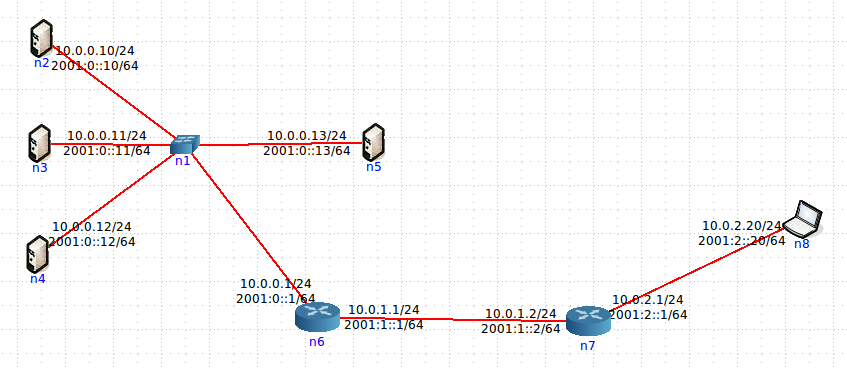
\includegraphics[height=6cm]{topologia.png}
\end{figure}
Numa primeira fase foi testada a comunicação UDP entre os UDPAgent's e o UDPMonitor através da execução de 3 UDPAgent's nas máquinas n2,n3 e n4 e o UDPMonitor na máquina n5 e observar o output resultante, como se pode observar de seguida:
\begin{figure}[H]
	\advance\leftskip-2cm
    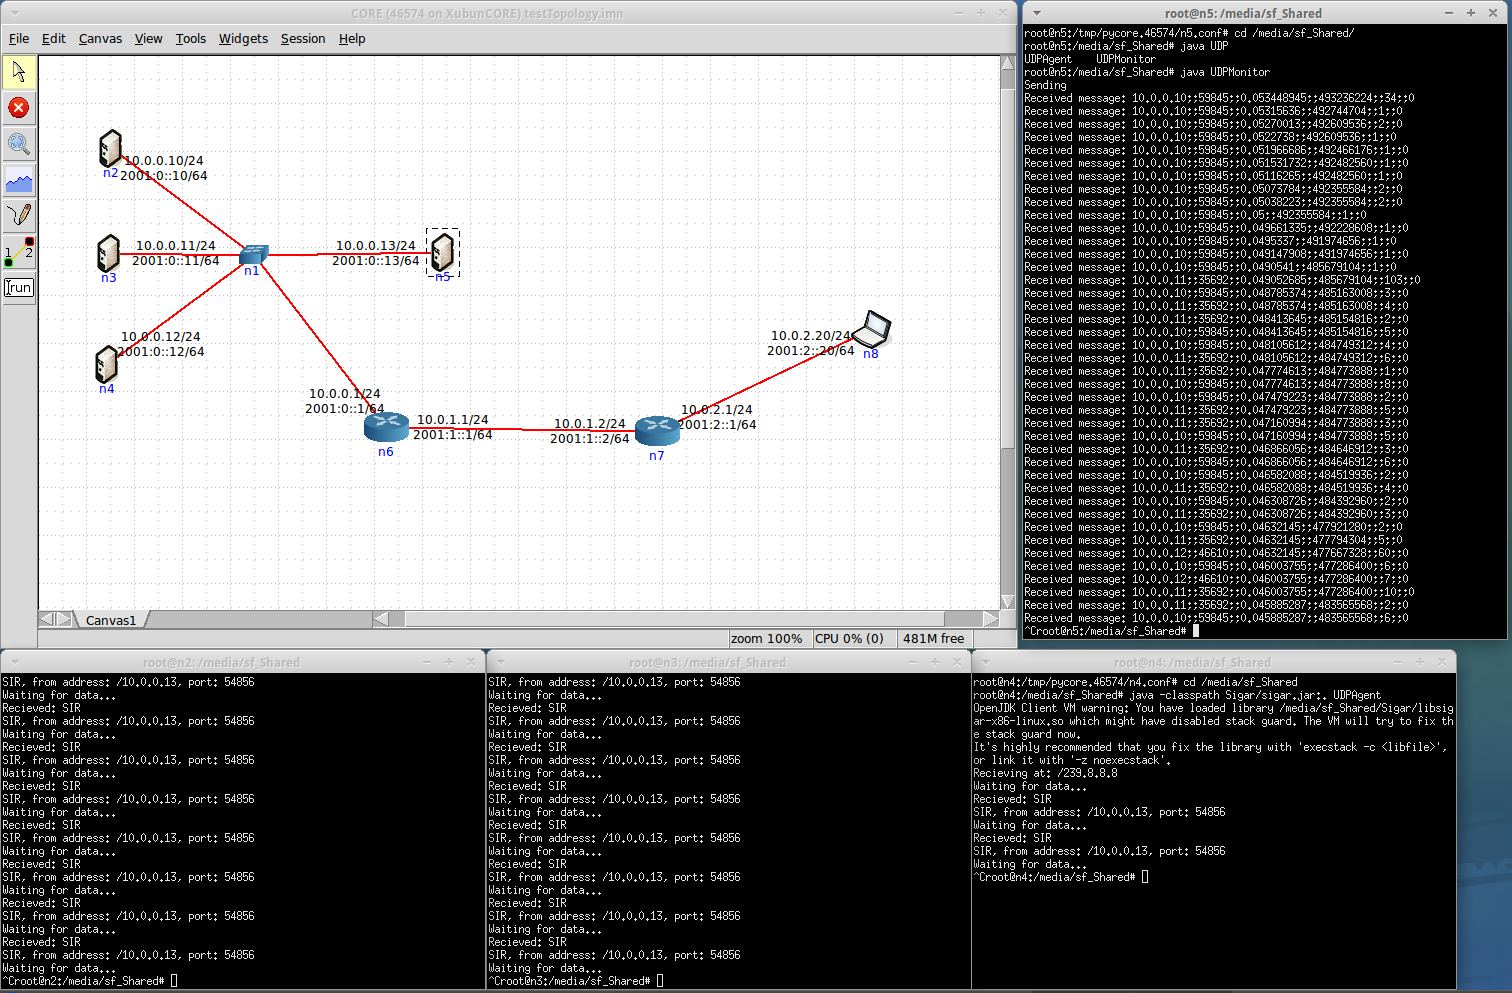
\includegraphics[height=11cm]{teste1.png}
\end{figure}

A compilação do código pode ser obtida executando as seguintes instruções:
\begin{verbatim}
$ javac UDPMonitor.java StateTable.java ReverseProxy.java
$ javac -classpath Sigar/sigar.jar UDPAgent.java
\end{verbatim}
O seguinte comando é usado para executar o Reverse Proxy bem como o UDPMonitor:
\begin{verbatim}
$ java UDPMonitor
\end{verbatim}
Já o UDPAgent nas outras máquinas deve ser executado da seguinte maneira:
\begin{verbatim}
$ java -classpath Sigar/sigar.jar:. UDPAgent
\end{verbatim}

Numa segunda fase foi testado o algoritmo de escolha do servidor HTTP por parte do Reverse Proxy bem como se a criação do canal entre o mesmo e o cliente era feito de forma transparente.
Como tal foi executado em cada máquina onde corre o UDPAgent (máquina n2, n3 e n4) o seguinte comando:
\begin{verbatim}
$ mini-httpd -d /srv/ftp/
\end{verbatim}
criando assim um servidor HTTP em cada uma que possui dois ficheiros que se podem descarregar. Para além disso é colocado a executar na máquina n5 o Reverse Proxy e o UDPMonitor.
Após isso é feito um pedido \texttt{wget} a partir do cliente com o endereço IP 10.0.2.20, por exemplo:
\begin{verbatim}
$ wget http://10.0.0.13/teste1Gb.db
\end{verbatim}
ao servidor Reverse Proxy (endereço IP: 10.0.0.13). Depois basta verificar se o ficheiro teste1Gb.db está presente no cliente e, em caso positivo, pode concluir-se que a operação funcionou corretamente. Ilustra-se na imagem seguinte o teste realizado:
\begin{figure}[H]
	\advance\leftskip-3cm
    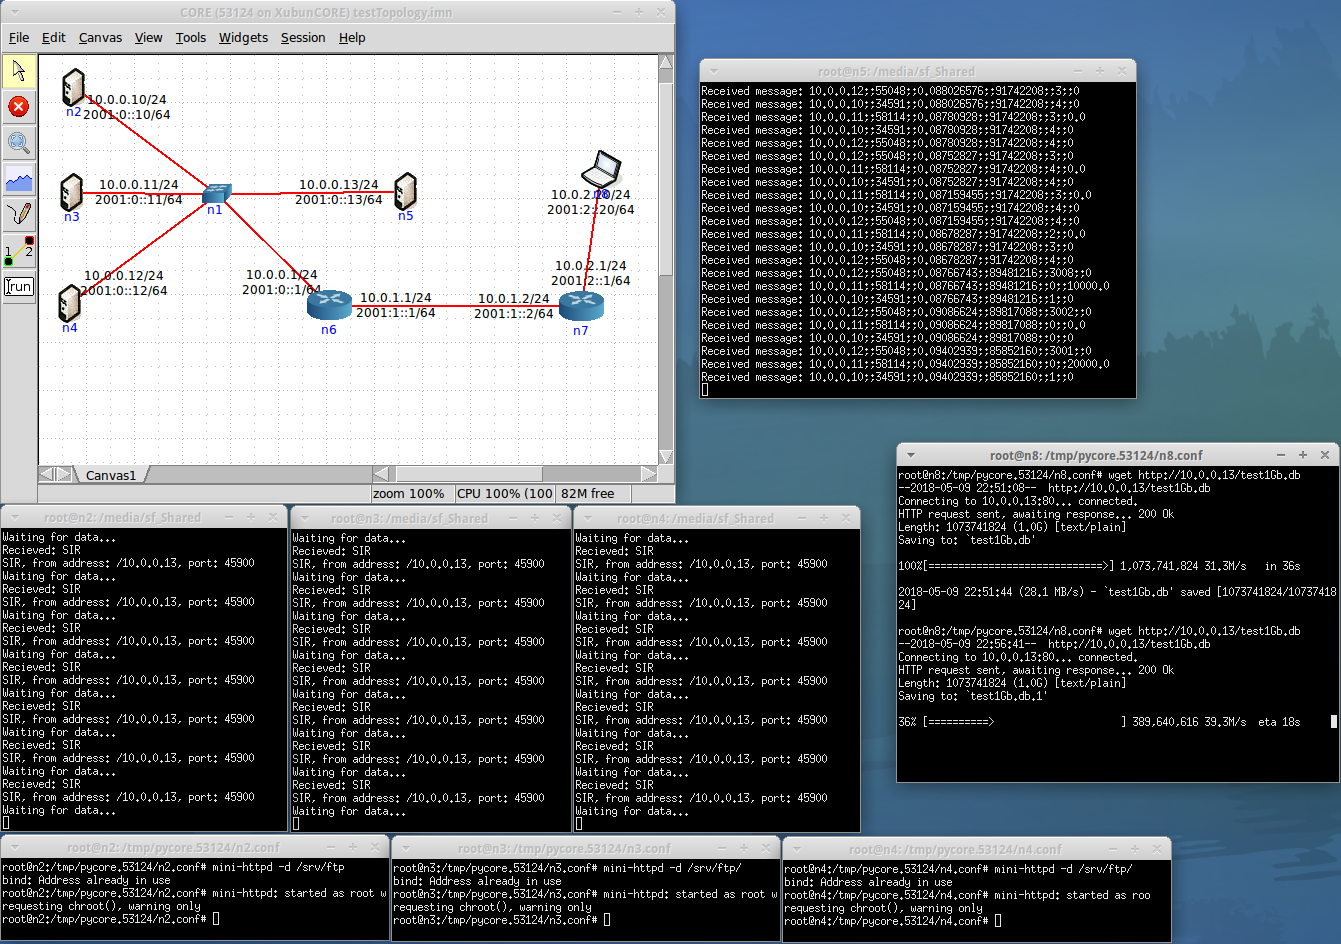
\includegraphics[height=13cm]{teste2.png}
\end{figure}

\section{Conclusões e trabalho futuro}
O trabalho realizado cumpre os requisitos propostos podendo, no entanto, ser melhorado, no sentido em que em vez do Reverse Proxy realizar a ligação entre o servidor back-end e o cliente, esta ligação seria estabelecida diretamente entre ambos enviando, para isso, o endereço do servidor back-end ao cliente evitando que se estabeleça um ponto de falha no Reverse Proxy.

\section{Lista de Siglas e Acrónimos}
\begin{description}
    \item [TCP] Transmission Control Protocol
    \item [UDP] User Datagram Protocol
    \item [HTTP] Hypertext Transfer Protocol
    \item [PDU] Protocol Data Unit
    \item [SIR] Server Information Request
    \item [SIRR] Server Information Request Response
    \item [PDU] Protocol Data Unit
    \item [Sigar] System Information Gatherer and Reporter
    \item [HMAC] Hash-Based Message Authentication Code
    \item [SHA] Secure Hash Algorithm
    \item [RTT] Round Trip Time
    \item [CORE] Common Open Research Emulator
\end{description}

\section{Referências}
Imagem na secção Arquitetura da Solução: Enunciado do Trabalho\\
Sigar Download: https://sourceforge.net/projects/sigar/\\
Sigar API: http://cpansearch.perl.org/src/DOUGM/hyperic-sigar-1.6.3-src/docs/javadoc/index.html\\
\end{document}
